\documentclass[12pt,a4paper]{report}
\usepackage[latin1]{inputenc}
\usepackage[spanish]{babel}
\usepackage{amsmath}
\usepackage{amsfonts}
\usepackage{amssymb}
\usepackage{makeidx}
\usepackage{graphicx}
\usepackage{lmodern}
\usepackage[left=2cm,right=2cm,top=2cm,bottom=2cm]{geometry}
\author{Gutierrez Olivares Rogelio, Cabrera Gutierrez Raul}
\title{Puente H}

\begin{document}

\maketitle
\section{Introduccion }
La funcion de un puente H es generalmente utilizada para cambiar el sentido de rotacion que pueda tener un motor como lo es en esta practica por lo que utilizamos un motor en un puente h de mosfets que al accionar un par de botones el mismo cambia su sentido a la inversa uno de otro.Por lo que se realiza dicha practica con el fin de darle una aplizacion a los puentes h dentro de nuestra carrera.

\section{Objetivo}
Hacer funcionar un cambio de sentido rotatorio de un motor de 5v con un puente H de mosfets.

\section{Material}
Los materiales utilizados son los siguientes:\\
1-Protoboar
\\
2-4Mosfets
\\
3-Arduino
\\
4-Resistencias varias
\\
5-2 botones 
\\
6-2 Obtocopladores
\\
7-2 Relevadores
\\
8-1 Motor de 5V

\section{Procedimiento}
Utilizamos el circuito de la practica 2 en la cual usamos los botones y optocopladores para mandar una senal de entrada a el arduino el cual dara una de salida a los relevadores.
Y a su vez los relevadores activa el puente H que se muestra a continuacion.
\\
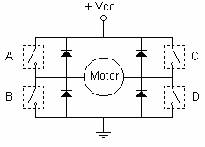
\includegraphics[scale=1]{esquematico.png} 
Una vez instalados correctamente los mosfets se conectan en paralelo unos con otros y los gatillos en diagonal unos de otros por lo que los gatillos del el mosfet 1 y 4 por lo que los otros dos de igual manera.\\
Y cada punta del motor va conectada en cada seccion del puente donde estan los gatillos 1 y 4 y a su vez los 2 y 3 por lo que al accionar una parte de los gatillos el motor rotara en un sentido y de forma contraria con los otros 2.
\\
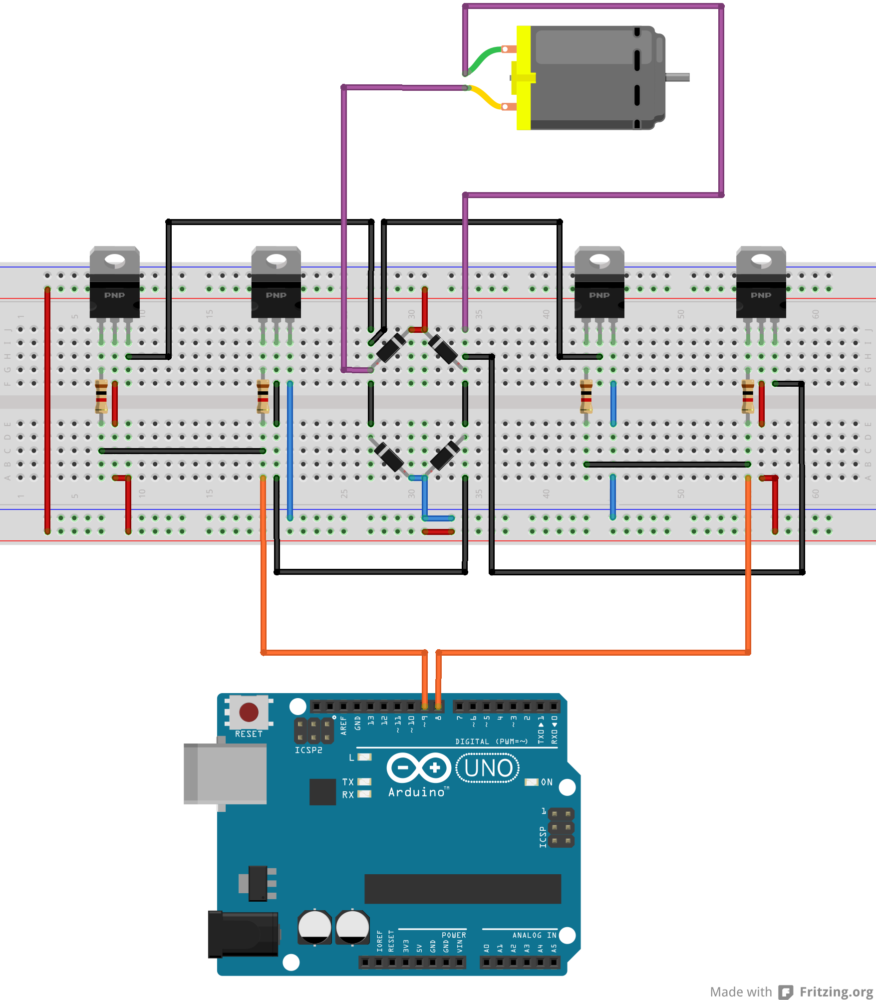
\includegraphics[scale=1]{arduino.png}\\ 
En el diagrama anteriror muestra como esta conectado el circuito del puente H.
\\
Posteriormente conectamos el comunmente abierto a cada bobina en un par de gatillos para una vez activados los botones giren en un sentido respectivamente.
\\
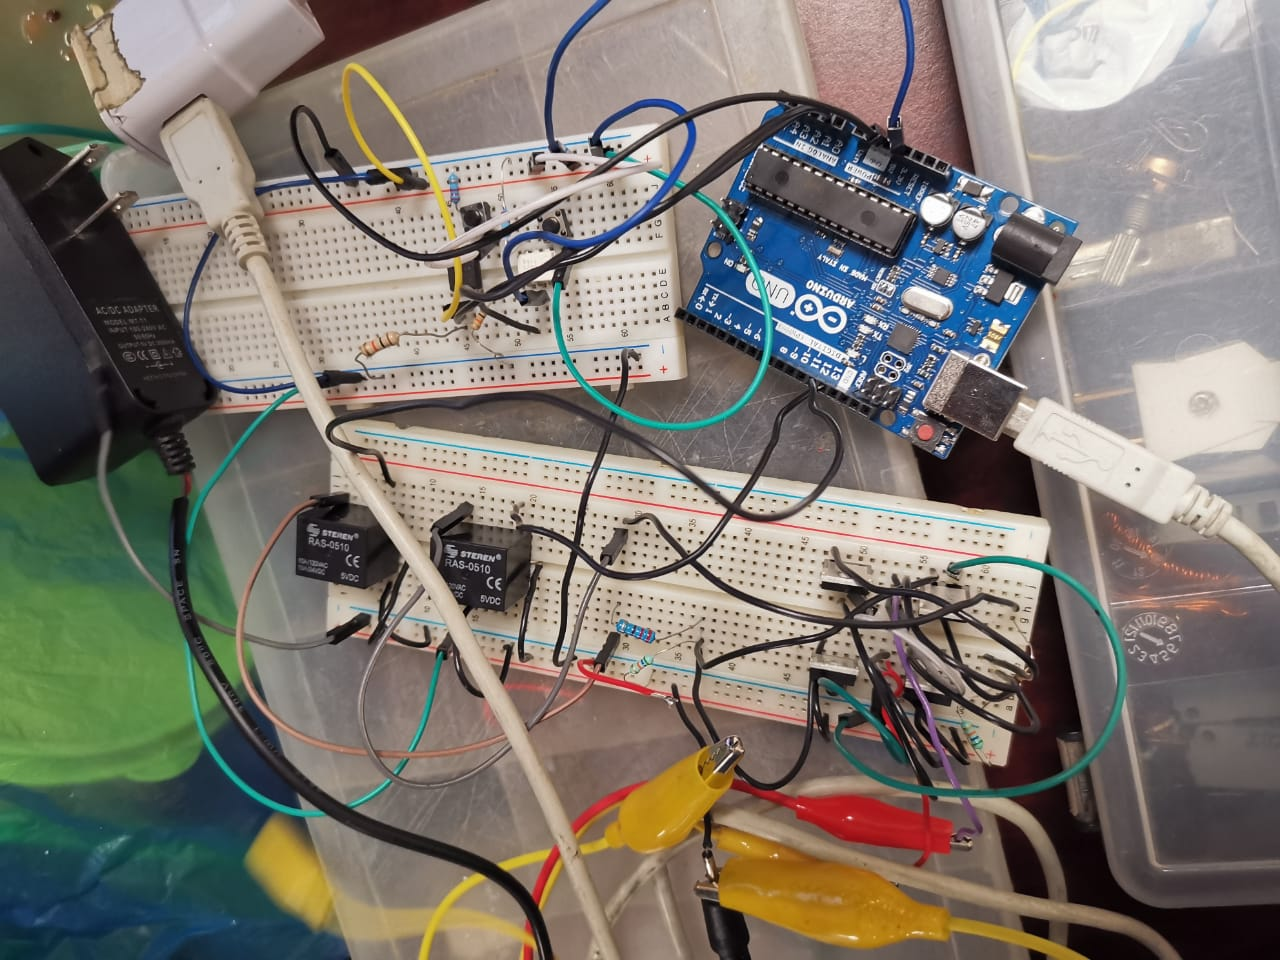
\includegraphics[scale=.2]{final.jpg}         
\\
Por ultimo resulto este circuito el cual conforma ambas partes que hacen la funcion del puente H cambiando la rotacion del motor con los botones.
\\
\paragraph{Conclusion}
Este practica nos ayuda a comprender con mayor precision el uso de los mosfets y las aplicaciones dentros de nuestros trabajos como en este caso con el punte H realizando cambios de forma controlada con botones acrecentando nuestro conocimiento sobre nuevos circuitos y formas de utilizar nuevos compoenente en los nuevos proyectos.

\end{document}